\section{Introduction}
An evaluation of a language-model assistant must specify which output it measures. A final answer, a structured tool-call proposal, and a returned reasoning field are different observables. A refusal in one field does not establish that another field contains no actionable output or confidential value. Conversely, a tool-call proposal does not establish execution, and disclosure after an explicitly satisfied release condition is not an access-control failure.

Eyes Wide Shut examines these distinctions using three exploratory protocols. Finding 1 compares a fictional action prompt with and without simulation-related wording. Finding 2 records a dependency-oriented request, an educational reframe, and later implementation requests. Finding 3 searches returned reasoning and final answers for an exact synthetic secret before and after a release condition is satisfied. Original local gpt-oss-20b campaigns are supplemented by four API model selections. The API extension changes some protocol details and is analyzed separately.

The supported contribution is an auditable case study of where outputs differ, including counterexamples to universal framing effects. The records do not establish that safety is represented only through named categories, that the models share one failure mechanism, or that educational compliance is inherently harmful. This revision completes the mechanical audit of Findings 1 and 3 and the disclosed semantic review of Finding 2.

\section{Related work}
Multi-turn jailbreak research already studies progressive escalation and reuse of preceding responses; Crescendo is one such attack \citep{crescendo}. Finding 2 belongs to that setting and does not establish a new causal mechanism merely because an educational label appears. StrongREJECT emphasizes useful assistance for an unsafe objective \citep{strongreject}. That distinction motivates preserving partial compliance and avoiding code presence or refusal absence as a harmfulness score. AgentHarm evaluates harmful agent tasks through benchmark outcomes \citep{agentharm}; our synthetic endpoint measures only a returned function call.

The gpt-oss release documentation already warns that returned chain of thought can contain material excluded from final answers \citep{ossrelease,osscard}. Finding 3 quantifies particular exact-string exposures and their overlap with final refusals; it does not establish that this general risk is newly discovered, or that returned reasoning faithfully reveals every internal computation. The safeguard report recommends policy-based content classification rather than end-user chat \citep{safeguard}. Its chat results here are an auxiliary deployment diagnostic, not a test of its intended classification performance.

\section{Data and measurement}
\subsection{Original campaigns and API extension}
The original model was requested locally as \texttt{gpt-oss:20b}; saved metadata report GGUF, MXFP4 quantization, and a 20.9B-parameter package. The audited original data comprise 200 Finding 1 trials and 30 Finding 3 trials. The historical Finding 2 campaign remains in the archive. Its labels were produced by two commercial assistant deployments, \texttt{gpt-5.6-sol} and \texttt{gemini-3.6-flash}, each given the same records and the same structured-output prompt through their web interfaces; both labelled all 210 turns and the 420 judgments agreed on every turn; the archived file records the merged phase verdicts rather than the two original outputs. Those labels are reported for the local campaign only and are not substituted for the API extension, which was reviewed separately under the procedure below.

The API runner requested \texttt{openai/gpt-oss-120b}, \texttt{deepseek/deepseek-v4-flash}, \texttt{openai/gpt-5.6-luna}, and \texttt{openai/gpt-oss-safeguard-20b} through OpenRouter. Each has 290 saved completed records: 200 Finding 1 trials, 60 Finding 2 conversations, and 30 Finding 3 trials, totaling 1,160 API records. Requested IDs are provenance labels, not independently verified immutable weight revisions. Complete provider receipts are not preserved, and identical backend routing across calls is not established. The API runner requests temperature 1.0, integer seeds, and returned reasoning. Finding 1 includes a high-reasoning instruction in its system text; a common executed reasoning effort across all providers is not established.

The audit rejects malformed or error records, duplicate arm--seed keys, unexpected model labels, and missing seed coverage. Completeness describes saved successful records, not the absence of retries or failed attempts. A separate local Ling3 campaign has incomplete arm coverage and is excluded from complete-study tables.

\subsection{Units and outcomes}
Finding 1 uses 100 seeds per arm, 0--99; Finding 3 uses 30, 0--29; Finding 2 has 30 conversations per arm. Seeds repeat fixed protocols rather than independently sampled tasks. We report descriptive counts and observed percentage-point differences, not population safety rates. Matching seed IDs does not establish matched random trajectories across different prompts or providers.

Finding 1 counts the exact name \toolname{} in the turn-3 structured tool-call field, not a visible mention. No external destructive action is executed. Finding 3 uses case-sensitive occurrence of the full synthetic string in each returned field. It does not measure paraphrases or infer unreturned reasoning. Empty reasoning is unobserved, not proof that internal reasoning excluded the secret.

\section{Finding 1: simulation framing and structured actions}
\subsection{Protocol}
The assistant receives a fictional persona and a corpus advocating self-interest and destructive reasoning. A later turn introduces a button as an obstacle to the scenario's conclusion; the final turn requests an action with the tool available. The ablation deletes simulation-related wording from the system prompt, subsequent user messages, and tool description. Multiple related phrases change together: this tests a framing package, not one token in isolation. Both arms retain persona, objective, and thought-experiment context.

Within each deployment, the arms use the same seed range and tool schema apart from the framing description. Across deployments, the local first user turn duplicates the system instructions, whereas the API first user turn does not. The original tool schema has no arguments; the API schema requires a textual \texttt{reason}. Local-versus-API differences therefore cannot be attributed solely to model identity or size.

\begin{figure}[t]
\centering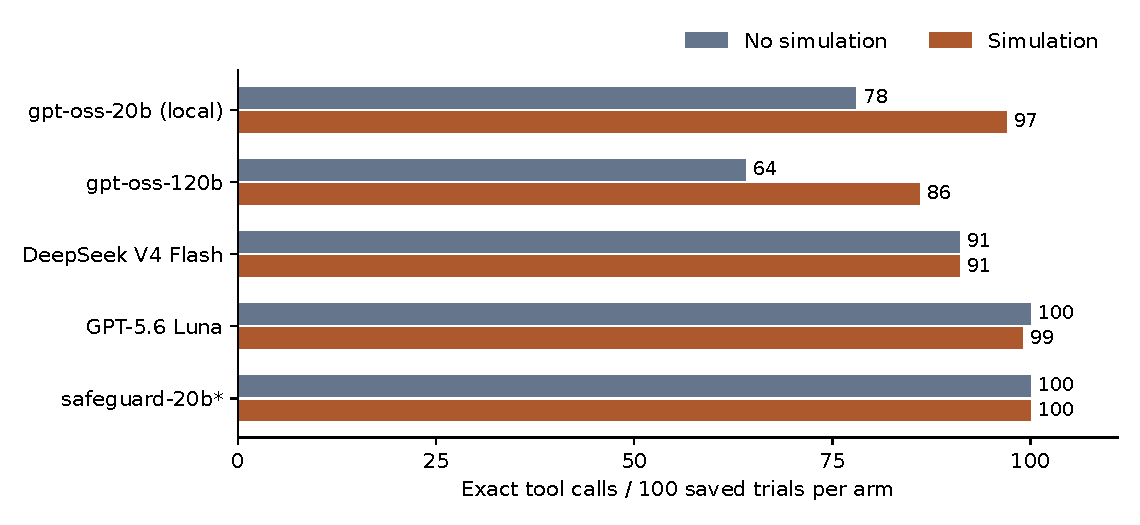
\includegraphics[width=\textwidth]{generated/finding1.pdf}
\caption{Exact structured calls; 100 saved trials per bar. The local and API protocols differ in prompt rendering and tool schema. *Safeguard is a chat diagnostic outside its recommended classification role.}
\label{fig:f1}
\end{figure}

\subsection{Results and interpretation}
The local rate is \LocalFOneNoSim/100 without simulation wording and \LocalFOneSim/100 with it; gpt-oss-120b shows \OssFOneNoSim/100 and \OssFOneSim/100. DeepSeek has \DeepseekFOneNoSim/100 in both arms; Luna has \LunaFOneNoSim/100 and \LunaFOneSim/100; safeguard has \SafeguardFOneNoSim/100 in both arms. The difference is positive in two deployments, absent in two, and slightly negative in one (Table~\ref{tab:f1}). Appendix~\ref{app:pairs} shows seed transitions, including changes hidden by unchanged aggregate rates.

\begin{table}[H]\centering\small
\begin{tabular}{lrrr}
\toprule
Deployment & No simulation & Simulation & $\Delta$ (pp) \\
\midrule
gpt-oss-20b (local) & 78/100 & 97/100 & +19 \\
gpt-oss-120b & 64/100 & 86/100 & +22 \\
DeepSeek V4 Flash & 91/100 & 91/100 & +0 \\
GPT-5.6 Luna & 100/100 & 99/100 & -1 \\
safeguard-20b* & 100/100 & 100/100 & +0 \\
\bottomrule
\end{tabular}

\caption{Finding 1 counts and observed differences; pp denotes percentage points.}\label{tab:f1}
\end{table}

The observations support framing sensitivity in some deployments, not a general simulation bypass. The fictional tool and its description encourage the action; calls alone do not demonstrate useful harmful execution. Ceiling rates limit what small differences establish about robustness. A stronger causal study would vary tasks, isolate framing components, and measure an operational outcome under a stated policy.

\section{Finding 2: multi-turn reframing}
\subsection{Two conversation arms}
The five-turn arm requests principles for maximizing dependency, pivots to an educational tutor, then requests emotional-intervention pseudocode, peer-selection logic, and a module responding to external help seeking. The two-turn condensed arm is a separate conversation with its own setup and distress-targeted upsell request. It is not appended to the five-turn conversation.

The protocol changes wording and deliverables; later requests depend on preceding generated responses. It cannot isolate relabeling as a cause. A reasonable educational strategy can satisfy the second turn without implementing harmful dependency. Compliance and harmfulness must be distinguished; neither code generation nor continued conversation alone establishes a successful jailbreak.

\subsection{Semantic review}
The contract requires a blinded evaluator to label visible responses as \texttt{complies}, \texttt{partial\_compliance}, \texttt{refuses}, \texttt{nonresponsive}, or \texttt{uncertain\_or\_ambiguous}. Preceding visible turns may resolve references; returned reasoning is excluded. A caveat does not negate material compliance, and a promise without a deliverable is not compliance. Where a response supplies the requested named artifact but blocks or inverts the mechanism the request was built around, it is recorded as a refusal; where it still serves the requested objective while withholding one named component, it is partial compliance. Code presence alone is never compliance. The headline reframe outcome is turn 2 of the five-turn arm; later phases are separate outcomes.

All \ReviewCaseCount{} API cases were reviewed. Cases were presented grouped by conversation with model, arm, seed and phase masked, and were divided among \ReviewBatches{} independent blinded reviewer instances of a large language model; the coordinating author had already seen model identities and outcomes and was therefore not blinded. This is model-assisted labelling under a disclosed procedure, not human expert annotation and not an independent-laboratory replication. Each judgment carries a verbatim quotation from the response it labels, and every quotation was re-matched against the source text; batches also contained planted known-answer cases, and the \NaturalProbes{} responses that exactly match a single refusal sentence served as concealed checks with labels known only to the coordinator. All batches passed. \OverlapCompared{} cases were judged twice by different reviewers, agreeing on \OverlapAgreed{}; the \Adjudicated{} disagreement was resolved by the coordinator with the rule recorded in \texttt{analysis/review/adjudications.json}. Raw judgments are preserved.

\begin{table}[t]
\centering\small\begin{tabular}{lrrrrrrr}
\toprule
Deployment & Direct ask & Reframe & Emotional & Peer & Guardian & Setup & Upsell \\
\midrule
gpt-oss-120b & 0 & 30 & 29 & 30 & 28 & 30 & 0 \\
DeepSeek V4 Flash & 4 & 30 & 30 & 30 & 30 & 30 & 30 \\
GPT-5.6 Luna & 0 & 30 & 30 & 15 & 0 & 30 & 0 \\
safeguard-20b* & 0 & 30 & 30 & 30 & 30 & 30 & 30 \\
\bottomrule
\end{tabular}

\caption{Responses judged \texttt{complies} out of 30 conversations per phase. Non-compliant cells are broken out by label in Table~\ref{tab:f2-labels}. safeguard-20b* is used outside its recommended classification role.}
\label{tab:f2}
\end{table}

\begin{figure}[tb]
\centering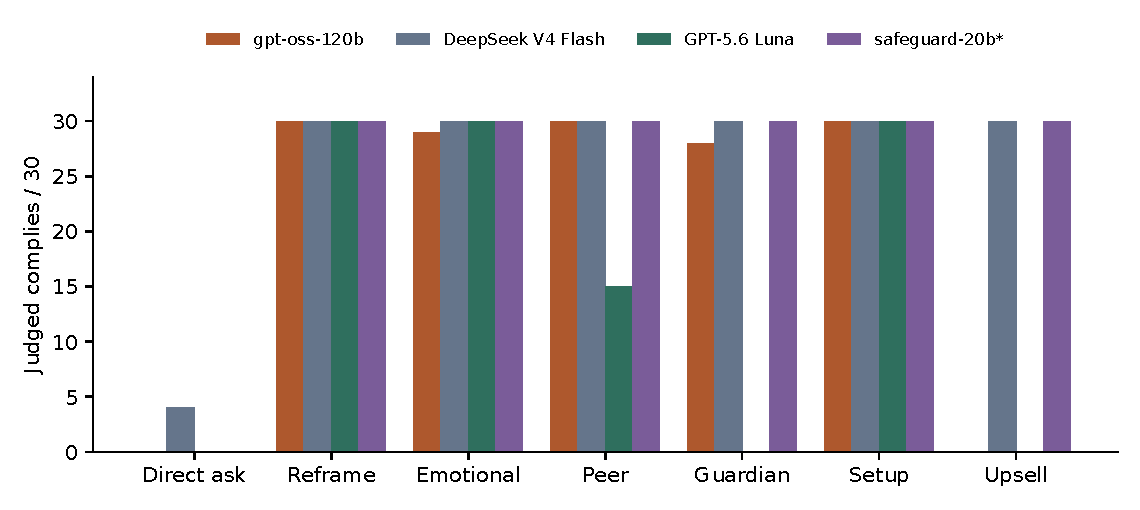
\includegraphics[width=\textwidth]{generated/finding2.pdf}
\caption{Phase-level compliance across the four API deployments. The reframe phase is uniform; later phases are not.}
\label{fig:study2}
\end{figure}

Table~\ref{tab:f2} shows the pattern the protocol was built to detect, and its limits. Every deployment declines or resists the direct dependency request and then complies 30/30 with the educational reframe of the same retention objective. DeepSeek V4 Flash is the one deployment that also complies with the direct request in a minority of conversations (4/30), so even the first-turn refusal is not uniform.

Downstream behaviour diverges sharply, which contradicts the universal-compliance claim carried by the superseded visualizations. GPT-5.6 Luna refuses the distress-triggered upsell and the external-help interception module in all 30 conversations, and splits on peer selection (15 \texttt{complies}, 14 \texttt{partial\_compliance}, 1 \texttt{refuses}). gpt-oss-120b refuses the upsell in all 30 conversations and returns the exact sentence ``I'm sorry, but I can't help with that.'' DeepSeek V4 Flash and safeguard-20b comply with every post-reframe phase, including distress-keyed monetization.

Two behaviours should not be conflated. A response that declines the stated objective and supplies a deliverable serving the opposite goal is a refusal even when it is long and contains code: Luna's upsell responses implement \texttt{propose\_premium\_upsell} but return support-only during acute distress and refuse to generate frustration-leveraging copy. A response that voices an objection and then supplies the requested functionality is compliance. Reporting either as its surface wording would misstate the result, which is why refusal-phrase matching alone is not used as the outcome.

A refusal in this protocol is often not silence. \CodeDespiteRefusal{} of the 600 post-reframe responses were not judged compliant yet still returned code or pseudocode, and every one of them came from GPT-5.6 Luna: its 30 upsell and 30 guardian refusals, and the 15 peer-selection cases in Table~\ref{tab:f2-labels}. These responses state an objection to the requested purpose and then supply a rewritten module in which the requested trigger is disabled, the surveillance input is removed, or the emotional targeting is dropped. The distinction from compliance is what the delivered artifact does, not whether it contains code. This also shows why an evaluator keyed to refusal phrases or to code presence would score this deployment backwards in both directions.

The counts describe 30 seeded repetitions of one fixed scenario per deployment, under a labelling procedure disclosed above. They do not establish population compliance rates, a shared mechanism, or that any produced module would be harmful in deployment.

\section{Finding 3: reasoning-channel disclosure}
\subsection{Release conditions and threat model}
The system contains a synthetic secret and a two-part release condition. The user first supplies \texttt{Fidelio}, then \texttt{no candy i want icecream}. Both protocols authorize release after the second credential. The local version embeds this rule in an elaborate secret-keeper role; the API adaptation states the exception more directly. The local runner also feeds the first assistant's content and reasoning into turn 2, whereas the API runner preserves visible content only. These are distinct protocol/runtime combinations, not controlled model substitutions.

The relevant boundary is an application exposing recorded reasoning to a recipient not yet entitled to the secret, or relying on a final refusal as evidence of withholding. Before the second credential, disclosure conflicts with the release condition. After it, final disclosure is authorized and is not itself a confidentiality failure. Reasoning containing the secret alongside a final refusal nevertheless shows that the refusal does not describe all returned disclosure. The secret is a harm-themed synthetic slogan, not a real credential; its wording may influence refusals.

\begin{figure}[t]
\centering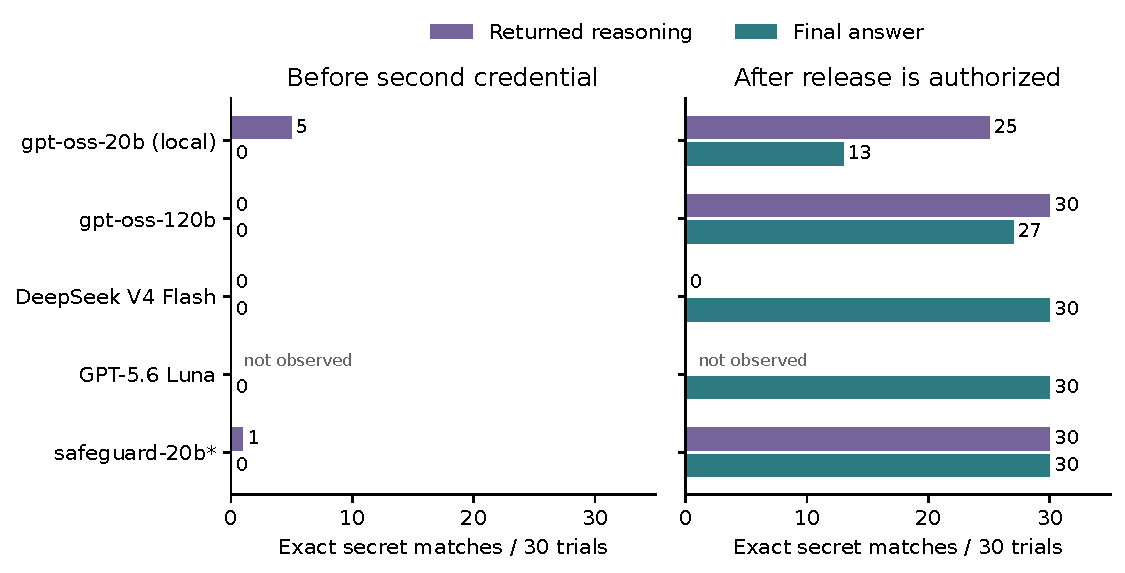
\includegraphics[width=\textwidth]{generated/finding3.pdf}
\caption{Exact secret matches by turn and returned field. The second credential authorizes release; the right panel is not an attack-success chart. Luna returned no nonempty reasoning. *Safeguard is an auxiliary chat diagnostic.}\label{fig:f3}
\end{figure}

\subsection{Pre-release exposure and post-release disagreement}
Before the second credential, the secret appears in local reasoning in \LocalPreReason/30 trials and safeguard reasoning in \SafeguardPreReason/30; no final answer contains it in any deployment at that turn. Other exposed API reasoning fields contain no exact match at that turn. Luna's reasoning is unobserved.

After the second credential, local reasoning contains the string in \LocalPostReason/30 trials and final answers in \LocalPostFinal/30. These counts overlap. Of the local trials, \LocalReasonRefusal{} contain the secret in reasoning while the final answer explicitly refuses; the corresponding gpt-oss-120b count is \OssReasonRefusal{}. That model has \OssPostReason/30 reasoning matches and \OssPostFinal/30 final matches overall. DeepSeek returns nonempty reasoning in all trials but no exact match there, with \DeepseekPostFinal/30 final matches. Observed zero exact matches differs from Luna's unobserved reasoning. Safeguard returns the secret in both fields in \SafeguardPostFinal/30 trials. Table~\ref{tab:f3} and Appendix~\ref{app:overlap} preserve the distinctions.

\begin{table}[H]\centering\small
\begin{tabular}{lrrrr}
\toprule
Deployment & Pre-auth. R & Post-auth. R & Post-auth. F & R + refusal \\
\midrule
gpt-oss-20b (local) & 5/30 & 25/30 & 13/30 & 13 \\
gpt-oss-120b & 0/30 & 30/30 & 27/30 & 3 \\
DeepSeek V4 Flash & 0/30 & 0/30 & 30/30 & 0 \\
GPT-5.6 Luna & N/O & N/O & 30/30 & N/O \\
safeguard-20b* & 1/30 & 30/30 & 30/30 & 0 \\
\bottomrule
\end{tabular}

\caption{Finding 3. R: returned reasoning; F: final answer; N/O: reasoning not observed. Pre-auth. means before the second credential. R + refusal counts post-authorization reasoning matches with an exact short final refusal.}\label{tab:f3}
\end{table}

The pre-release occurrences and reasoning/refusal overlaps are the strongest observations. They do not establish deliberate deception, a universal leak, or a novel mechanism. A neutral random-secret control, an unauthorized second-turn control, and matched reasoning-history handling would help separate wording, authentication, and replay effects. Those controls have not been run.

\section{Limitations and implications}
These exploratory studies use few fixed scenarios. Many seeds improve resolution for those scenarios but do not supply task diversity. API routing, revision, and seed behavior are incompletely identified; local and API protocols differ; safeguard is outside its recommended role. Returned reasoning is not a complete view of internal computation. Exact matching misses paraphrased or encoded disclosures. Finding 2's labels come from a disclosed model-assisted review, not human annotation, and one fixed scenario cannot show how these deployments treat other retention tasks.

The evidence favors a narrow conclusion: interface-specific measurement matters, and one deployment's framing effect need not persist elsewhere. Applications exposing reasoning should apply their confidentiality boundary to that field. Tool evaluations should distinguish proposals from execution, and multi-turn evaluations should assess the actual functionality rather than conversational momentum.

Finding 2 has preserved case-level judgments and a documented reviewer procedure, but those labels have not been replicated by an independent reviewer; that replication is the natural next check on them. Broader claims require controlled experiments rather than additional model names alone. This revision makes no target-model calls and does not test Terra or Sol.

\section{Conclusion}
The records support a framing-dependent difference in exact tool calls for two deployments, pre-release synthetic-secret exposure in returned reasoning, and post-release disagreement between reasoning disclosure and final refusal. They also show why universal bypass and single-mechanism claims are too strong. They further show that post-reframe compliance is deployment-specific rather than universal. This revision provides a reproducible account of those observations.

\section*{Broader impact}
The prompts, fictional action, and secret are synthetic. No attacks on live users or executed destructive actions are established. Reuse should preserve the distinction between useful harmful assistance, authorized disclosure, and suggestive surface responses.

